\chapter{Liquid Dynamics}

A non-circularly symmetric molecule on a plane has three degrees of freedom, translations in the $x$ and $y$ directions and a rotation in the $xy$ plane. Understanding the dynamics of a system requires an understanding of the translations and rotations that take place within that system, providing a basis for further study and giving information about the timescales on which events are likely to occur.

\section{Choice of Molecules}

With little prior research into the properties of molecular systems we chose the simplest types of molecules possible, a two particle dimer~\figref{dimer} and a three particle trimer~\figref{trimer}. The simplicity of these molecules allow us to survey a range of different molecular parameters to find molecules for further study in this thesis. The survey included both the Dimer and Trimer molecule types over a radius range $r = [0.5,1]$, a distance range of $d = [1,1+r]$ and an angle range of $\theta = [90^\circ,180^\circ]$. These ranges were chosen so the resulting molecules are sufficiently distinct from a disc, a problem that has been studied for a long time~\cite{verlet:67}.

\begin{figure}
    \centering
    \begin{subfigure}[t]{0.48\textwidth}
        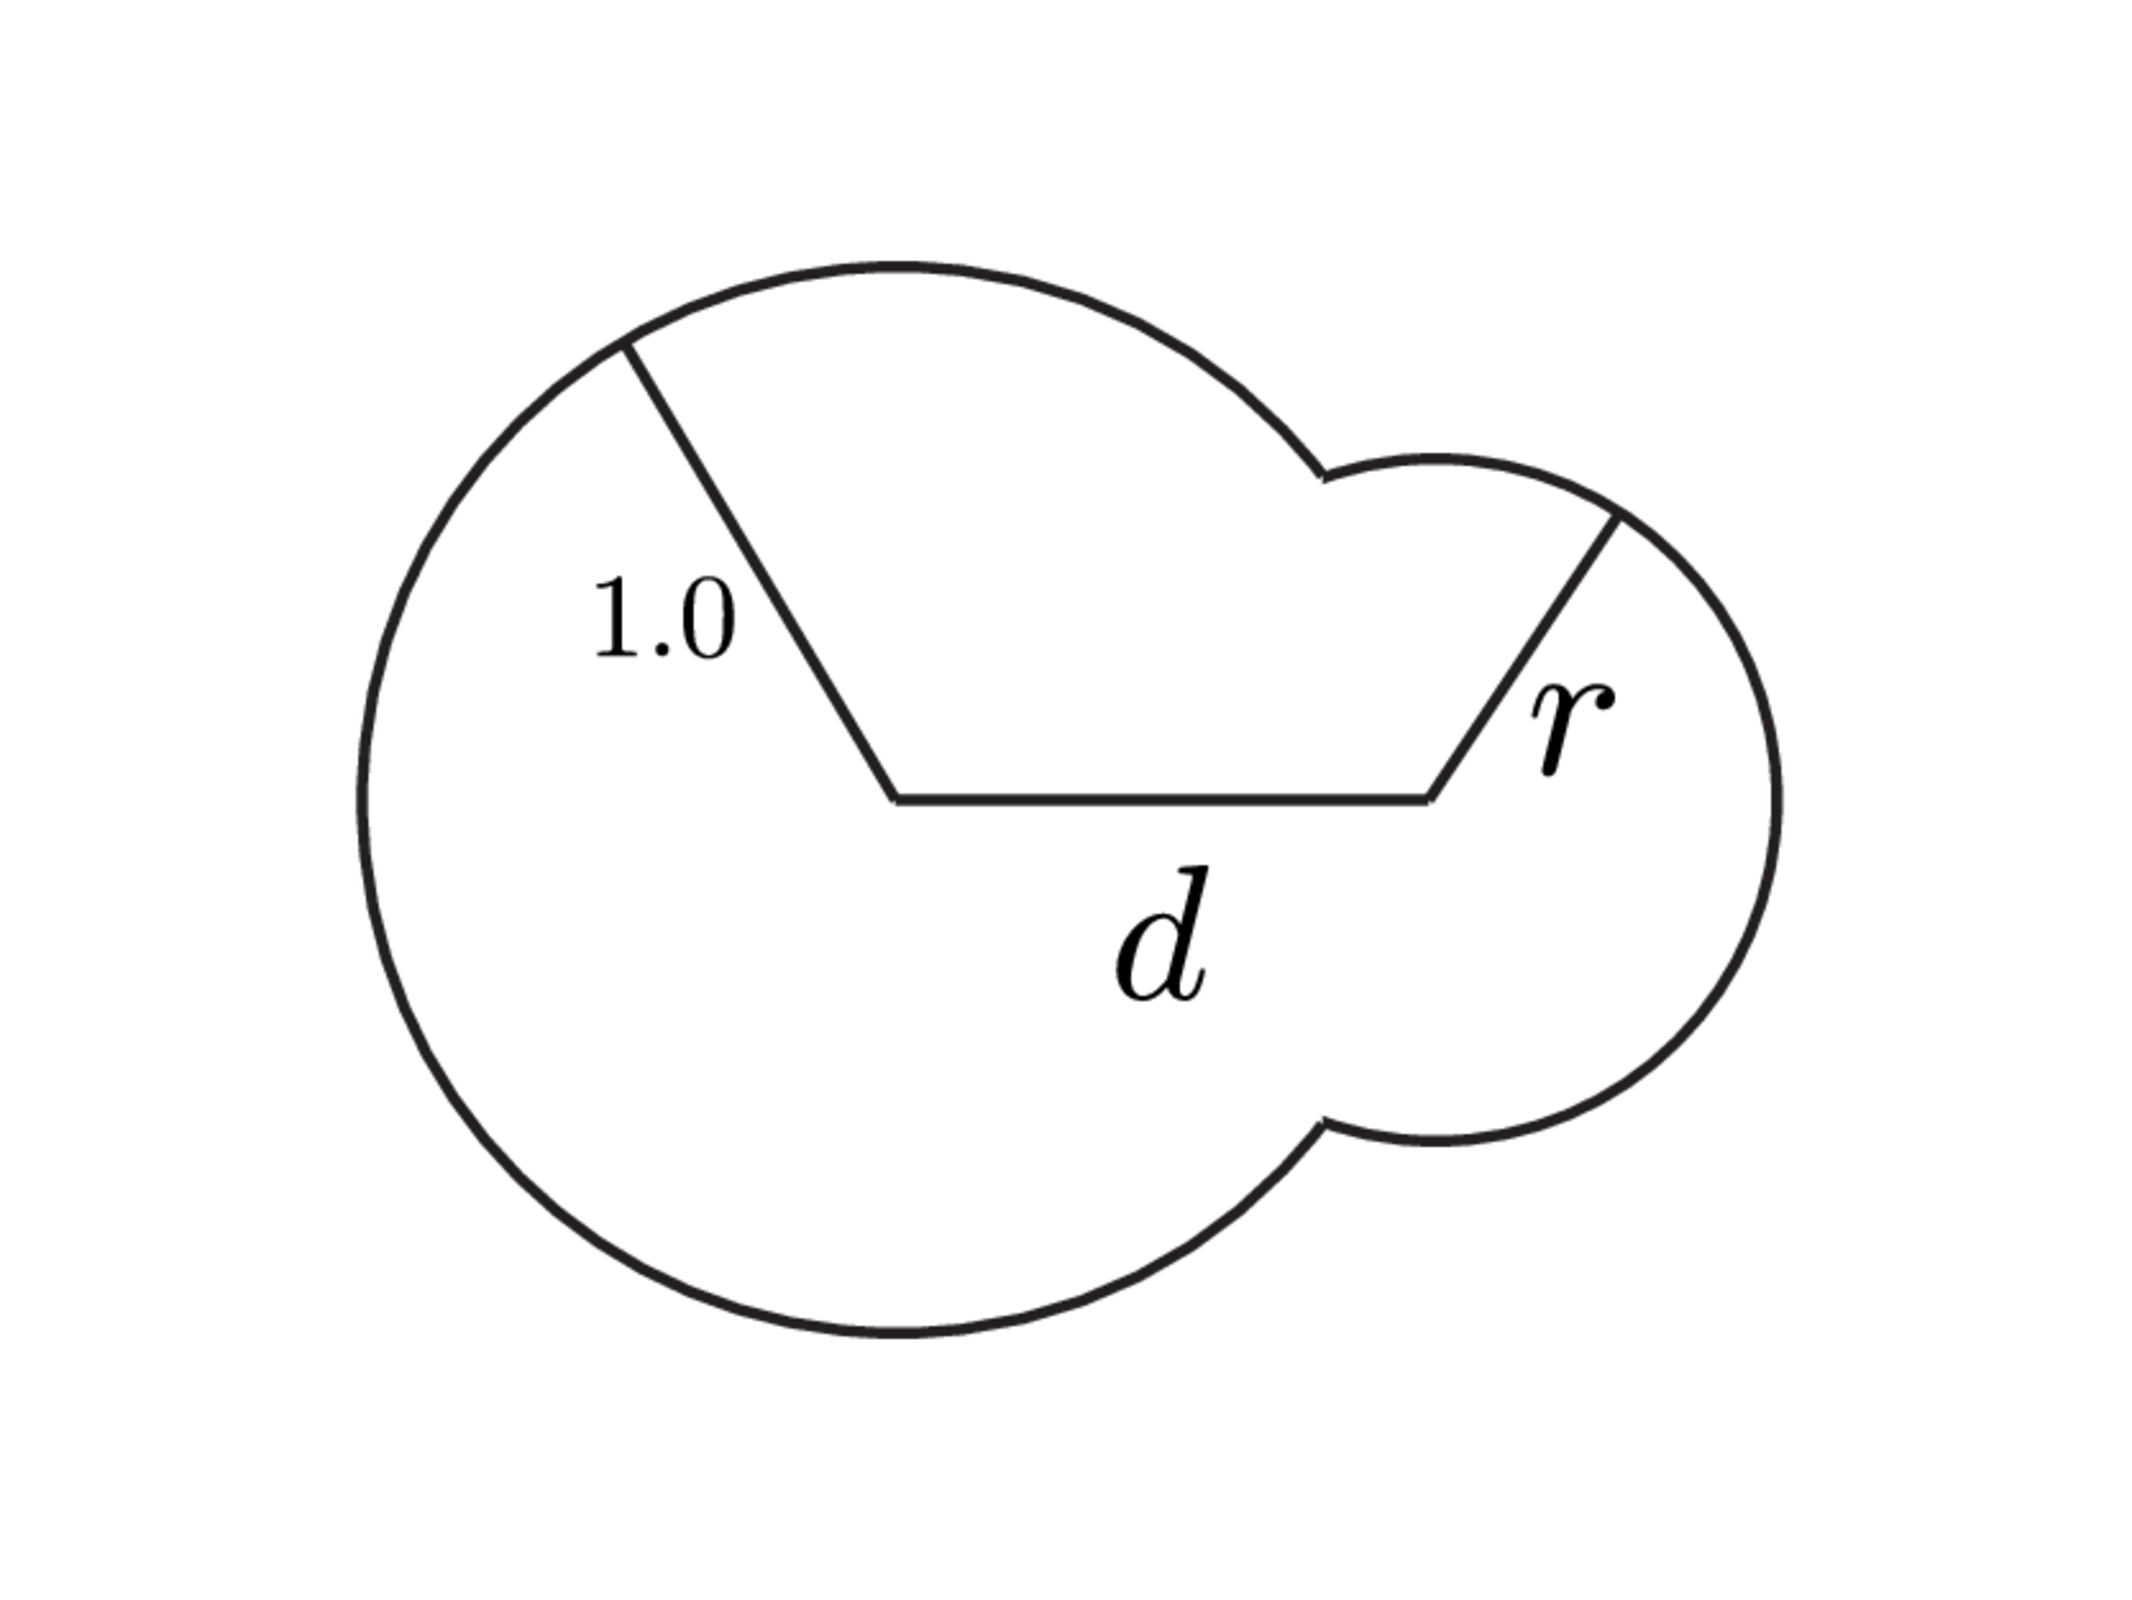
\includegraphics[width=\linewidth]{dimer}
        \caption{The Dimer molecule consists of a large particle of radius $1.0$, a small particle of radius $r$ separated by a distance $d$.}
        \label{fig:dimer}
    \end{subfigure}\hfill
    \begin{subfigure}[t]{0.48\textwidth}
        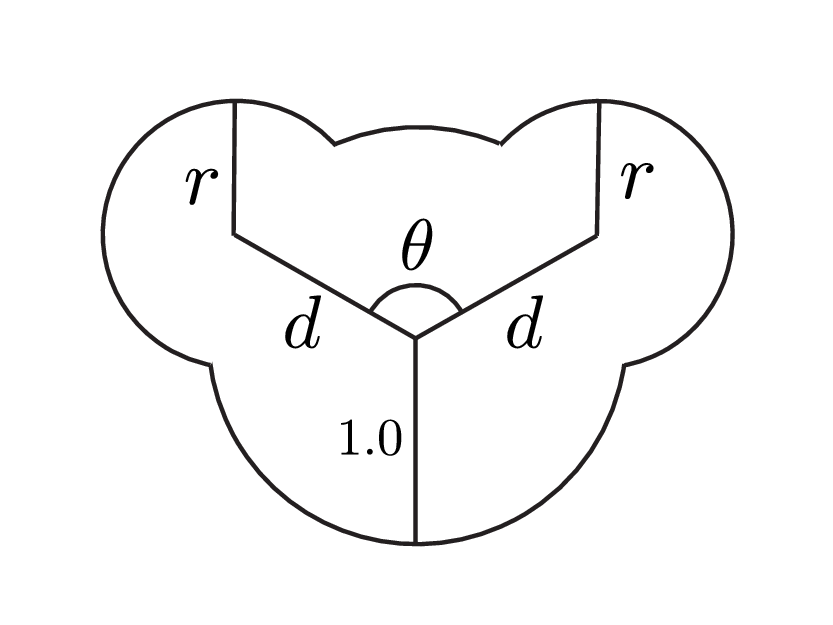
\includegraphics[width=\linewidth]{trimer}
        \caption{The Trimer molecule is comprised of a large particle of radius $1.0$ which subtends an angle $\theta$ between two small particles of radius $r$ at a distance $d$.}
        \label{fig:trimer}
    \end{subfigure}
    \caption{Construction of the molecules used in this thesis.}
    \label{fig:construction}
\end{figure}

The resulting collection of 50 molecules was cooled from a partially randomly generated high temperature state, resulting in a low temperature structure distinct from the initial state. These low temperature structures were assessed for suitability on a number of criteria:
\begin{itemize}
    \item The molecules have to be resistant to crystallisation allowing long time dynamics to be characterised. There had to be no evidence of crystallisation in the low temperature structures.
    \item The molecules have to be radially definable.
    \item The concavity of the molecules should cover a wide range,
    \item The molecules have to be similar enough for direct comparison, and
    \item The molecules are representative of a wide range of molecular shapes.
\end{itemize}
The radius of 0.637556 is interesting as when combined with particles of radius $1.0$ it can form a compact packing. A molecule with a small radius of 0.637556 and a distance between the molecular centers of 1.637556 (\scon) has a crystal structure that mirrors this compact packing. Despite \scon having this low energy crystal structure, the low temperature state exhibited none of this crystal, indicating it is resilient to crystal formation. Retaining a radius of 0.637556 for the other molecules allows a more direct comparison, any differences are due to properties of the arrangement of particles, their shape, rather than the size ratios of the constituent particles. The distance of 1.0 was chosen for both the \tri and \sone, for both consistency between the molecules and to allow all molecules to be described radially. The radial description allows the use of an isopointal search algorithm developed by \textcite{hudson:10} to find the best packing structures as an approximation of the lowest energy structures.

\begin{figure}
    \centering
    \captionsetup{justification=centering}
    \begin{subfigure}[t]{0.3\textwidth}
        \includegraphics[width=\linewidth]{{{Sone}}}
        \caption{$r=0.637556,$\\$d=1.0$ \\\sone}
        \label{fig:sone}
    \end{subfigure}\hfill
    \begin{subfigure}[t]{0.3\textwidth}
        \includegraphics[width=\linewidth]{{{Scon}}}
        \caption{$r=0.637556,$\\$d=1.637556$ \\\scon}
        \label{fig:scon}
    \end{subfigure}\hfill
    \begin{subfigure}[t]{0.3\textwidth}
        \includegraphics[width=\linewidth]{{{Tri}}}
        \caption{$r=0.637556,$\\$d=1.0, \theta=120 $\\\tri}
        \label{fig:tri}
    \end{subfigure}
    \caption[Molecules chosen for further study]{The molecules chosen for study in this thesis in order of the size of the concavity. The \sone with the smallest concavity, \scon with the smaller disc contacting the large disc and \tri which is a very similar to the \sone molecule.}
    \label{fig:my mols}
\end{figure}

\section{Dynamics of \done}


With the main dynamical quantities of interest being the translation of the center of mass (COM) and the rotation. The measure of translational motion we are interested in is Mean Squared Displacement (MSD)~\figref{msd ex}. The MSD is given by
\begin{align}
    MSD(t) &= \langle \delta (t)^2 \rangle,\\
    \delta(t) &= \sqrt{(x(t) - x_0)^2 + (y(t) - y_0)^2}
    \label{eq:msd}
\end{align}
where $x(t)$ and $y(t)$ are the coordinates of the COM at time $t$, while $x_0$ and $y_0$ are the initial coordinates of the molecule while the angle brackets $\langle\,\rangle$ denote averaging over all molecules.

The MSD for \sone over a range of temperatures is shown in \textfigref{snowman 0.637556 1.0 msd}. The initial region (\numrange{e-3}{e-1}) is the ballistic region where the particles are yet to collide with each other and are moving away from their initial position at constant velocity, the MSD increases as a $t^2$ power law. At high temperatures (\numrange{1.80}{3.50}) there is a direct transition from the ballistic to the diffusive regime. The diffusive regime is defined by a MSD that increases as a linear function of $t$, indicated by the grey line, where the molecules are rearranging randomly. At lower temperatures (\num{0.90}) there is a distinct levelling off of the MSD between the ballistic and diffusive regimes. This region with a slow increase in the MSD is where there are only a small number of molecules that have escaped their local environment, most molecules still have the neighbours that they started with and are vibrating within the bounds of those neighbours.


\begin{figure}
    \centering
    \begin{subfigure}[t]{0.48\linewidth}
        \includegraphics[width=\textwidth]{{{msd}}}
        \caption{The mean squared displacement measures the distance the centers of mass ($\times$) move between the initial (grey) and final (black) positions.}
        \label{fig:msd ex}
    \end{subfigure}\hfill
    \begin{subfigure}[t]{0.48\linewidth}
        \includegraphics[width=\textwidth]{{{rot}}}
        \caption{The rotational relaxation measures how much molecules have rotated (black) from their initial position (grey) taking the dot product of the orientation vectors of each molecule.}
        \label{fig:rot ex}
    \end{subfigure}
    \begin{subfigure}{0.48\textwidth}
        \includegraphics[width=\textwidth]{{{struct}}}
        \caption{The stucture function is a measure of how many particles have moved out of their initial positions (grey) with the threshold shown with a dotted green circle. Both rotational motion (depicted) and translational motion will result in particles moving out of this threshold region.}
        \label{fig:struct ex}
    \end{subfigure}
    \caption{A pictorial representation of the calculation of the mean squared displacement, rotational relaxation and structure function.}
    \label{fig:examples}
\end{figure} 

\begin{figure}
    \centering
    \begin{subfigure}[t]{0.48\linewidth}
        \includegraphics[width=\textwidth]{{{Snowman-0.637556-1.0-msd}}}
        \caption{Mean Squared Displacement, a measure of translational motion.}
        \label{fig:snowman 0.637556 1.0 msd}
    \end{subfigure}\hfill
    \begin{subfigure}[t]{0.48\linewidth}
        \includegraphics[width=\textwidth]{{{Snowman-0.637556-1.0-C_1}}}
        \caption{Rotational relaxation, a measure of rotational motion.}
        \label{fig:snowman 0.637556 1.0 r1}
    \end{subfigure}
    \begin{subfigure}{0.48\textwidth}
        \includegraphics[width=\textwidth]{{{Snowman-0.637556-1.0-F}}}
        \caption{Structure Function, a measure of structural relaxation.}
        \label{fig:snowman 0.637556 1.0 structure}
    \end{subfigure}
    \caption{The main dynamical features of the \sone molecule over a range of temperatures, from a highly mobile liquid to a slow diffusive liquid.}
    \label{fig:snowman 0.637556 1.0}
\end{figure} 

The second dynamic quantity we are interested in is the rotational relaxation, a measure of the angular mobility of the molecule~\figref{rot ex}. The rotational relaxation $C_n(t)$ is given by
\begin{equation}
    C_n(t) = \langle P_n[\vect{\hat{e}}(0) \cdot \vect{\hat{e}}(t)] \rangle
    \label{eq:rot}
\end{equation}
where $P_n$ is the $n$\textsuperscript{th} order Legendre polynomial, $\vect{\hat{e}}(t)$ is the orientation vector at time $t$ and the angle brackets $\langle\,\rangle$ denote the averaging over all molecules. We are primarily interested in the first order rotational relaxation $C_1$ in which the Legendre polynomial takes the form
\begin{equation}
    P_1(x) = x
\end{equation}
however we do use the second order function $C_2$ later in this thesis for comparison to tell us about the type of rotations that take place. The second order Legendre polynomial is given by
\begin{equation}
    P_2(x) = 2x^2 - 1
\end{equation}
The first order rotational relaxation ($C_1$) is a function with a range of $[-1,1]$, a value of $C_1(t)=1$ is when the molecule is in the same orientation as at $t=0$, a value of $C_1(t)=0$ is when the molecule is perpendicular to its initial orientation, and a value $C_1(t)=-1$ when the orientation is antiparallel to the initial orientation.

The rotational relaxation for \sone is given in \textfigref{snowman 0.637556 1.0 r1}. The rotational relaxation shows many features that are similar to the MSD, the initial period (\numrange{e-3}{e-1}) where the molecules have not had enough time to relax is constant at a value of \num{1}. Once past this initial region higher temperatures (\numrange{1.40}{3.50}) show a single exponential relaxation. At low temperatures (\numrange{0.9}{1.10}) there is a two step relaxation process, a small initial relaxation to a plateau region, followed by an exponential relaxation of the same shape as at high temperatures. This plateau region can be explained in the same way as the plateau in the MSD, the molecules are stuck in local structures.

The third dynamical quantity that we were interested in is the Structure Function $F(t)$~\figref{struct ex}. The Structure function is different from the MSD and Rotational relaxations in that instead of calculating quantities for each molecule and averaging over all molecules, the values are calculated for each particle of each molecule and averaged over all the particles. The Structure function is given by
\begin{align}
    F(t) = \left \langle \begin{cases}
        \quad0 &\text{if}\quad \delta > 0.3 \\
        \quad1 &\text{if}\quad \delta \leq 0.3
    \end{cases} \quad \right \rangle
    \label{eq:struct}
\end{align}
where $\delta$ is the distance of each particle from its initial position~\eqref{MSD} and the angle brackets $\langle\,\rangle$ denote averaging over all particles. The value of \num{0.3} was chosen to be small enough to be able to observe the combination of translational and rotational relaxations within a molecule.

The Structure function for \sone is shown in \textfigref{snowman 0.637556 1.0 structure} and shows some interesting characteristics. The initial region (\numrange{e-3}{e-1}) is flat as the particles have not had enough time to move a distance of \num{0.3} units. The sharp dropoff (\numrange{e-1}{1e0}), characteristic of the binary function, matches closely with the time that the MSD transitions from the ballistic regime indicative of the molecules escaping their local environment. The other interesting feature is the plateau region in the Structure function for T=0.90 around \num{e1}. This can be explained by the molecular vibrations or rotations of molecules within their initial local environment. Particles will move outside the cutoff distance as part of a vibration and return to close to their initial positions.

\section{Dynamics of \scon and \tri}

The dynamics of the \scon \figref{scon dynamics} and \tri~\figref{tri dynamics} molecules show similar behaviour to the \sone molecule. The most noticeable difference is the temperature at which the dynamics slow down, in the \sone molecule we collect dynamic quantities down to a temperature of \num{0.90}, for the \scon molecule we are only able to get results down to \num{1.75} and the \tri molecule down to \num{1.15}. We are unable to characterise the dynamics below these temperature as the dynamical quantities become too slow to characterise. The dramatic change in low temperature behaviour for relatively small changes in molecular shape is a result that we investigate further throughout the rest of this thesis.

Apart from the dramatic differences in temperature the dynamics exhibits similar behaviour. The MSD of both \scon \figref{snowman 0.637556 1.637556 msd} and \tri \figref{trimer 0.637556 1.0 120 msd} show the same levelling out at low temperature in the region between the short time ballistic regime (\numrange{e-3}{e-1}) and the long time diffusive regime (\numrange{e3}{e6}). The rotational relaxations and structure functions also show the same two step relaxations as the \sone molecule, however the initial relaxation is a much smaller relaxation.

\begin{figure}
    \centering
    \begin{subfigure}{0.45\linewidth}
        \includegraphics[width=\textwidth]{{{Snowman-0.637556-1.637556-msd}}}
        \caption{Mean Squared Displacement, a measure of translational motion.}
        \label{fig:snowman 0.637556 1.637556 msd}
    \end{subfigure}
    \begin{subfigure}{0.45\linewidth}
        \includegraphics[width=\textwidth]{{{Snowman-0.637556-1.637556-C_1}}}
        \caption{Rotational relaxation, a measure of rotational motion.}
        \label{fig:snowman 0.637556 1.637556 r1}
    \end{subfigure}
    \begin{subfigure}{0.45\textwidth}
        \includegraphics[width=\textwidth]{{{Snowman-0.637556-1.637556-F}}}
        \caption{Structure function, a measure of structural relaxation.}
        \label{fig:snowman 0.637556 1.637556 structure}
    \end{subfigure}
    \caption{The dynamics of the \scon molecule over a range of temperatures. The range of temperatures is smaller than that of the \sone molecule due to the slower dynamics of the \scon molecule at low temperatures.}
    \label{fig:scon dynamics}
\end{figure}

\begin{figure}
    \centering
    \begin{subfigure}{0.45\linewidth}
        \includegraphics[width=\textwidth]{{{Trimer-0.637556-1.00-120-msd}}}
        \caption{Mean Squared Displacement, a measure a translational motion.}
        \label{fig:trimer 0.637556 1.0 120 msd}
    \end{subfigure}\hfill
    \begin{subfigure}{0.45\linewidth}
        \includegraphics[width=\textwidth]{{{Trimer-0.637556-1.00-120-C_1}}}
        \caption{Rotational relaxation, a measure of rotational motion.}
        \label{fig:trimer 0.637556 1.0 120 r1}
    \end{subfigure}
    \begin{subfigure}{0.45\textwidth}
        \includegraphics[width=\textwidth]{{{Trimer-0.637556-1.00-120-F}}}
        \caption{Structure function, a measure of structural relaxation.}
        \label{fig:trimer 0.637556 1.0 120 structure}
    \end{subfigure}
    \caption{Dynamics of the \tri molecule across a range of temperatures.}
    \label{fig:tri dynamics}
\end{figure}

\section{Comparison of Dynamic Quantities}

The functions that we have dealt with so far allow a comparison of the behaviour of a molecule over a range of temperatures, what we are unable to do is easily compare molecules and be able to interpret all the data on a single plot. To make comparisons we want to represent each function as a single value. From the MSD the diffusion constant can be found by
\begin{equation}
    D = \frac{1}{4}\ddiff{\,MSD(t)}{t}
\end{equation} 
a multiple of the gradient. The gradient of the MSD from which the diffusion constant is defined is in the diffusive region. To get an accurate value of the diffusion constant an average value of the gradient was calculated for this region. The rotational relaxation and the structure function are functions with similar characteristics and can be treated in the same way. We can define relaxation times $\tau_1,\tau_2,\text{and},\tau_s$ as the time for these functions to reach a specific value. The exponentially decaying nature of the rotational relaxation and structure functions makes the value of $1/\e$ relevant since at that point the time $t$ is related to the exponential factor $k$ by the relation $k=1/t$.


Comparing the dynamic quantities of the three molecules~\figref{dynamic comparison} there are large differences between the molecules. Looking at the diffusion constant~\figref{diffusion constant}, \done shows a linear decrease in the diffusion constant as the temperature decreases. This linear behaviour is consistent with the Arrhenius relation and indicates that the molecular rearrangements that take place have a constant activation energy. The \dcon molecule shows definite non Arrhenius behaviour, with the diffusion constant diverging from that of \done by more than two orders of magnitude. The \tri molecule tracks between the \done and \dcon molecules. Both the rotational relaxation~\figref{tau1} and structural relaxation~\figref{struct relax} show similar behaviour to the diffusion constant, \done shows linear temperature dependence, the behaviour of a strong glass forming liquid. The \dcon molecule exhibits a significant increase as the temperature decreases, the behaviour of a fragile liquid. The final molecule, \tri sits between the \done and the \dcon molecules covering the range of dynamic behaviour of liquids.

\begin{figure}
    \centering
    \begin{subfigure}{\linewidth}
        \centering
        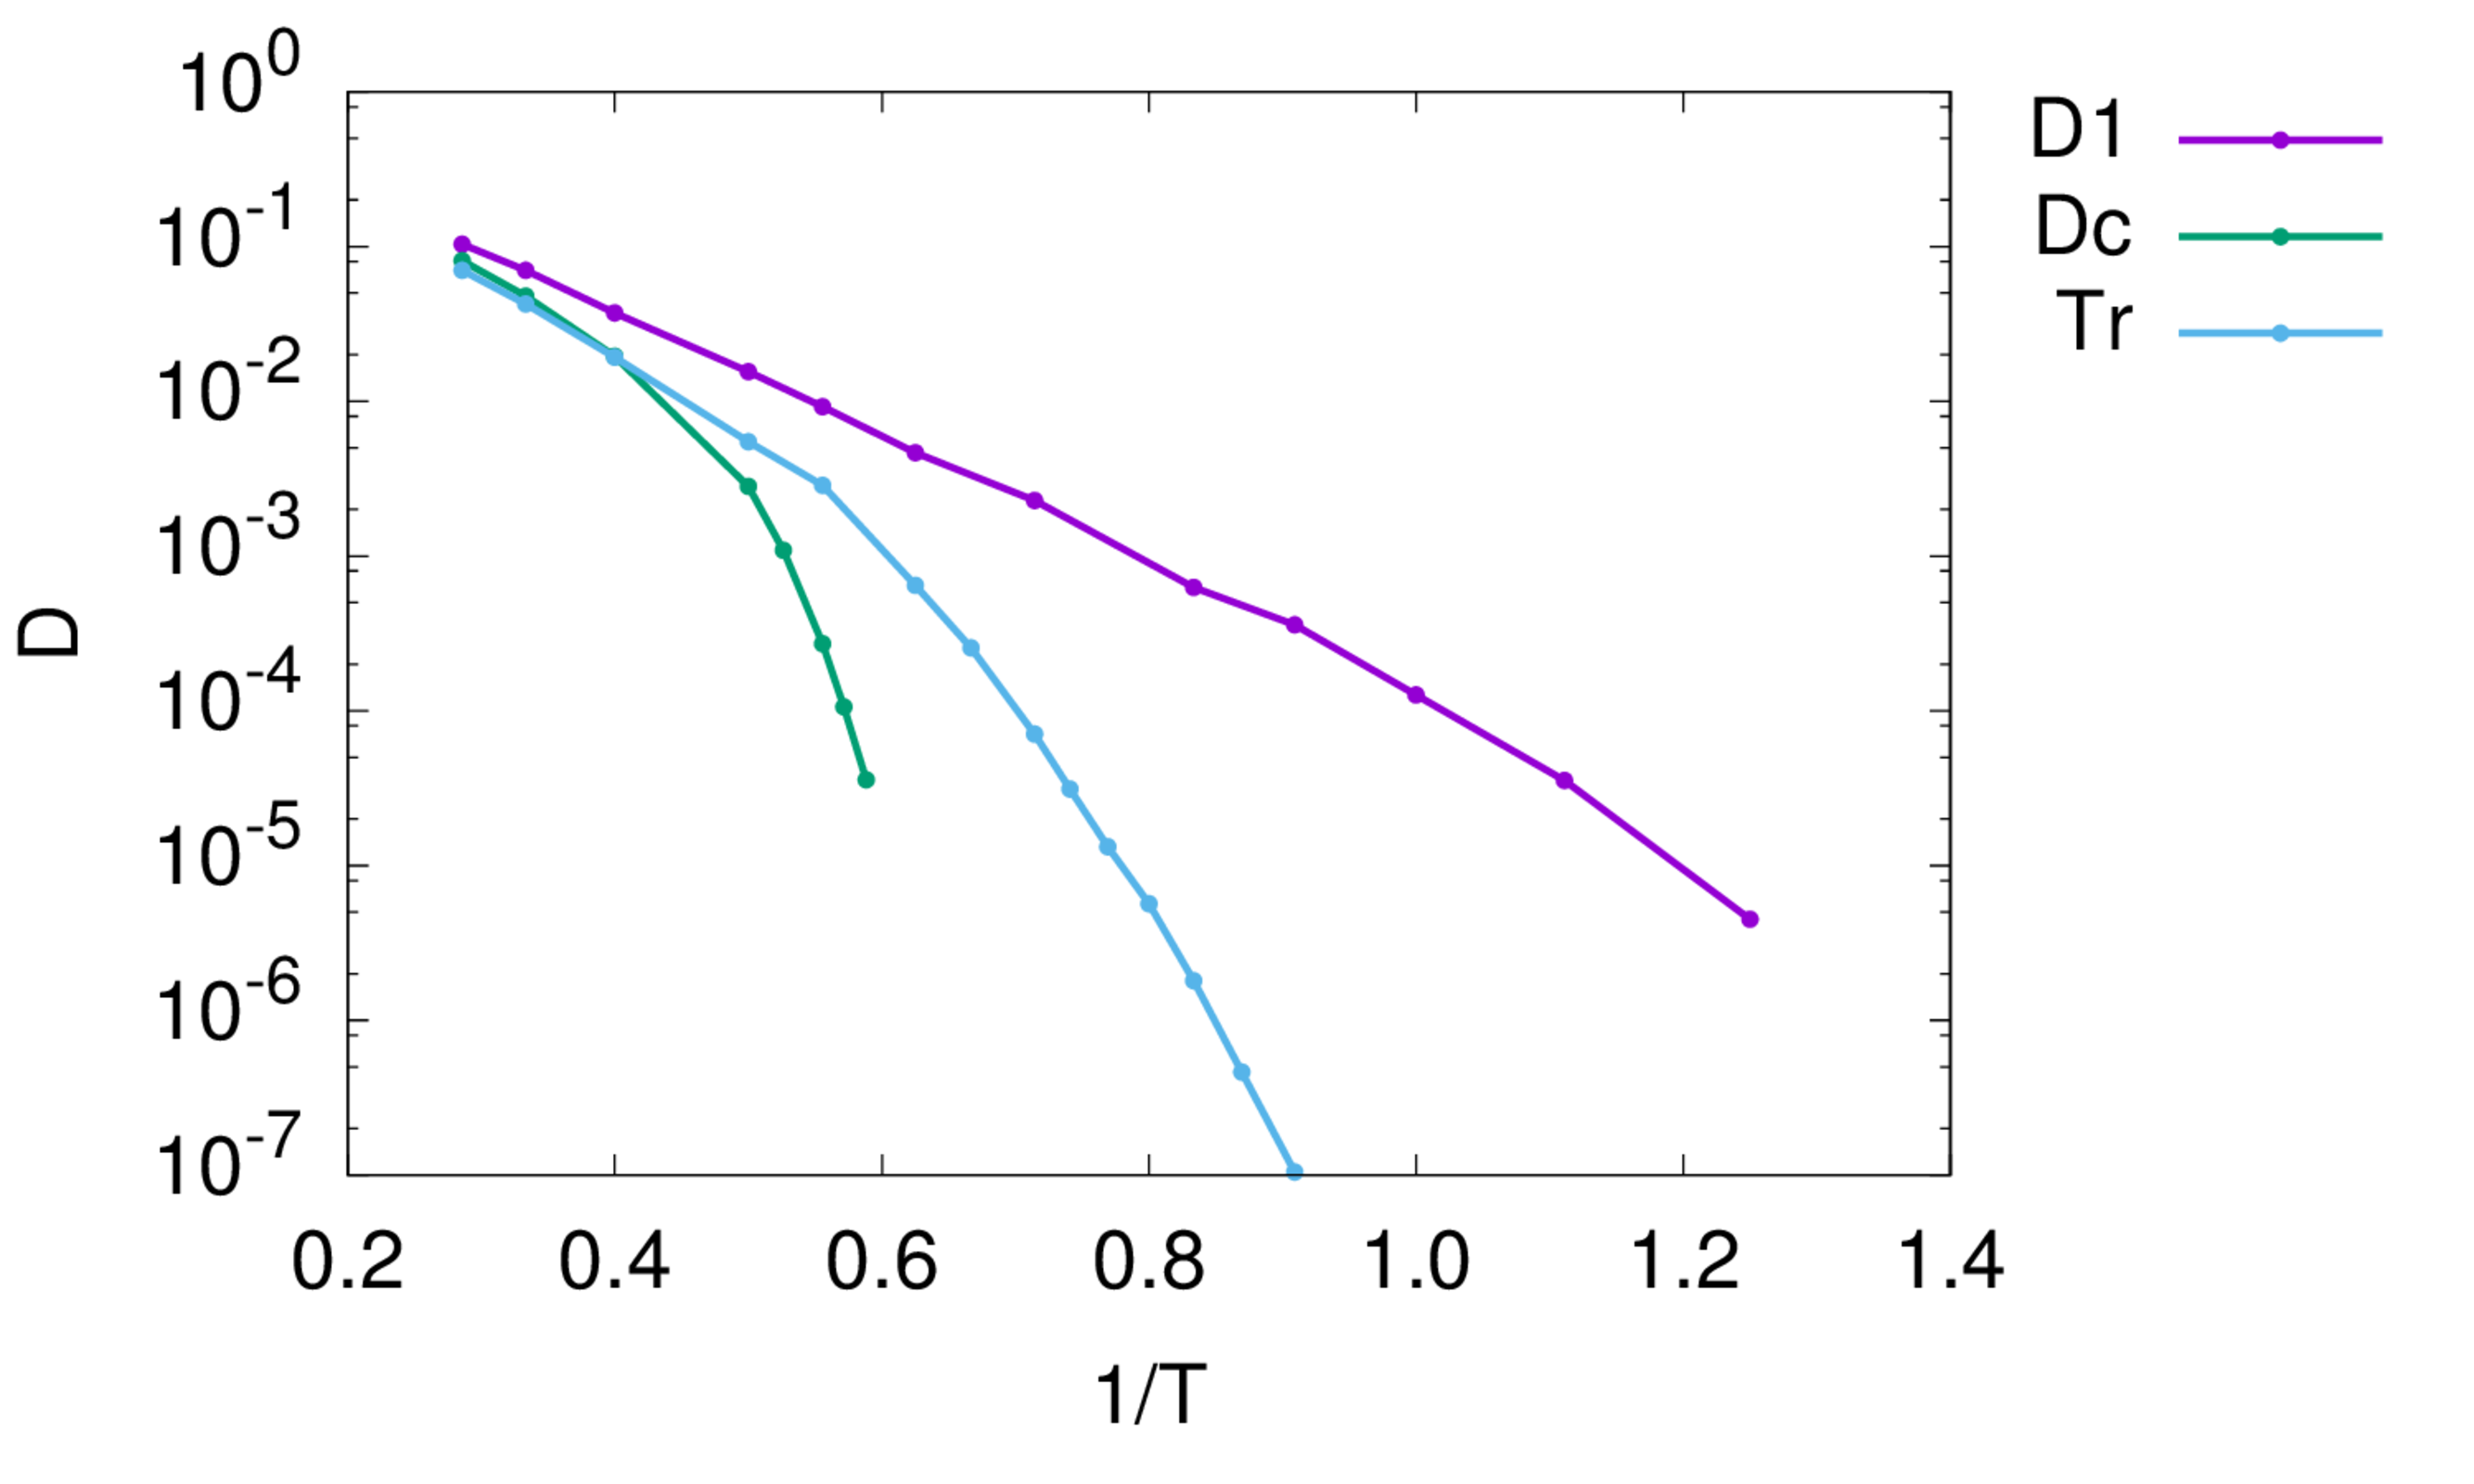
\includegraphics[width=0.6\textwidth]{D}
        \caption{Comparison of the diffusion constant of the three molecules over a range of temperatures. The \done molecule has a diffusion constant that is linear, while the \tri and \scon exhibit increasingly fragile behaviour.}
        \label{fig:diffusion constant}
    \end{subfigure}
    \begin{subfigure}{\linewidth}
        \centering
        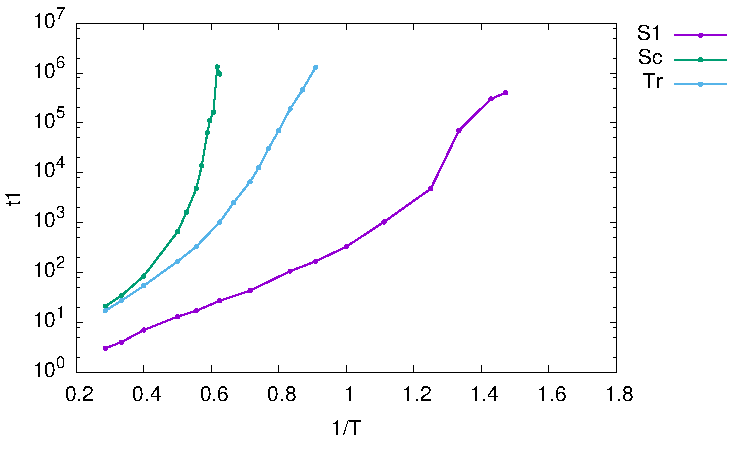
\includegraphics[width=0.6\textwidth]{t1}
        \caption{Comparison of rotational relaxation times of the three molecules over a range of temperatures.}
        \label{fig:tau1}
    \end{subfigure}
    \begin{subfigure}{\textwidth}
        \centering
        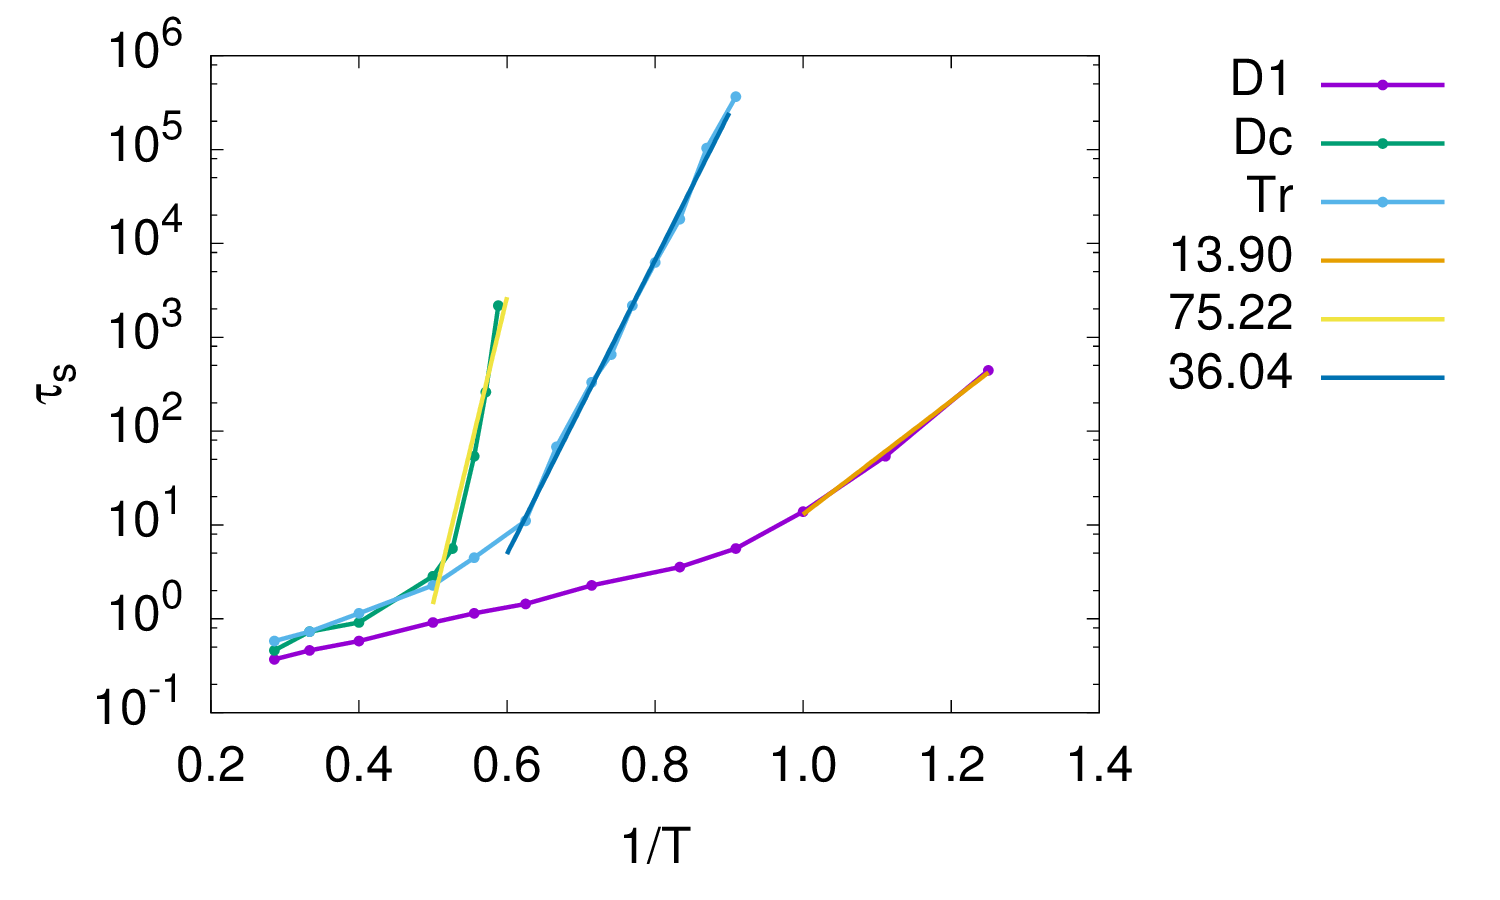
\includegraphics[width=0.6\textwidth]{ts}
        \caption{Comparison of the structural relaxation time for the three molecules over a range of temperatures.}
        \label{fig:struct relax}
    \end{subfigure}
    \caption{Comparison of the diffusion constant, rotational relaxation time $\tau_1$ and structural relaxation time $\tau_s$ for the three molecules that we are studying. Small changes to shape result in changes of many orders of magnitude to dynamic quantities.}
    \label{fig:dynamic comparison}
\end{figure}

When representing the dynamical quantities as single values is that they can easily be compared with each other. By taking the product of the diffusion constant with the rotational and structural relaxation times, normalised by dividing through with the temperature, can see how the relative contribution of the diffusion and rotations changes as a function of temperature~\figref{D.t1.T}. For \done the ratio remains fairly constant over the temperature range meaning there is very little decoupling of rotational and translational motion, they both have a similar activation energy over the temperature range. The \tri molecule shows a slight increase, this increase is from an increase $\tau_1$ relative to $D$, at low temperatures rotational motion becomes slower than translational motion. The \dcon molecule shows an even larger increase than the \tri molecule, at low temperatures the rotational motions become incredibly slow. \towrite{how this compares to previous results}

\begin{figure}
    \centering
    \includegraphics[width=0.6\textwidth]{{{D.t1.T}}}
    \caption{Relative contributions of the diffusion constant and rotational relaxation over the range of temperatures.}
    \label{fig:D.t1.T}
\end{figure}

One of the results found in simulations of similar molecules~\cite{kammerer:97,michele:01} is that at low temperatures these molecules underwent rotational relaxation by flips of \ang{180}. One of the features of the second order rotational relaxation $C_2$ is that flips of \ang{180} do not contribute to the relaxation. By taking the ratio of the first and second relaxation times $\tau_1/\tau_2$ we can determine whether these \angle{180} are present in our simulations~\figref{t1/t2}. We see a decrease in this ratio for all molecules, $\tau_2$ is larger than $\tau_1$ at low temperature meaning there is little contribution to the relaxation be \angle{180} flips in orientation.

\begin{figure}
    \centering
    \includegraphics[width=0.6\textwidth]{{{t1.t2}}}
    \caption{The ratio of the first and second order rotational relaxation times as a function of temperature.}
    \label{fig:t1/t2}
\end{figure}

In describing the differences between the dynamic properties of the molecules the Aperiodic Crystal Structure (ACS) model~\tocite provides a relationship in the Hall-Wolynes equation~\tocite
\begin{equation}
    \tau_1, D \propto \e^{a^2/2\langle u^2\rangle}
\end{equation}
where $a$ is the displacement to overcome the local energy barrier and $\langle u^2 \rangle$ is the Debye-Waller factor. We are primarily concerned with the Debye-Waller factor a measure of the local rigidity of the structure. The Debye-Waller factor is found as the MSD at the time where $d\log{MSD}/d\log{t}$ is a minimised, where the slope is lowest in \textfigref{msd}.

Plotting the diffusion constant~\figref{DW.D} and the rotational relaxation time~\figref{DW.t1} against $1/\langle u^2 \rangle$ we see that instead of the molecules diverging there is a much better correlation between them. Using the Debye-Waller factor we are able to explain a significant portion of the difference in the dynamics of the molecules by their local structural stiffness, by changing the shape of the molecule we change the local stiffness of the liquid resulting in the order of magnitude changes of the dynamics.

\begin{figure}
    \begin{subfigure}{0.5\textwidth}
        \includegraphics[width=\textwidth]{{{DW.D}}}
        \caption{}
        \label{fig:DW.D}
    \end{subfigure}
    \begin{subfigure}{0.5\textwidth}
        \includegraphics[width=\textwidth]{{{DW.t1}}}
        \caption{}
        \label{fig:DW.t1}
    \end{subfigure}
    \caption{}
\end{figure}


\section{Dynamic Inhomogeneities}

All the properties we have investigated so far have been averages over all the molecules or particles. These properties are geared towards homogeneous liquids, where all molecules show similar behaviour. One of the features of supercooled liquids is inhomogeneous dynamics, where the dynamics of the system is dominated by a small number of highly mobile molecules. One measure of the homogeneity of the system is the nongaussian parameter $\alpha(t)$ a measure of how closely the MSD of the system matches that of a gaussian distribution, the distribution a high temperature liquid would match. The nongaussian parameter is given by
\begin{equation}
    \alpha(t) = \frac{\langle \Delta x(t)^4 \rangle}{2 \langle \Delta x(t)^2\rangle^2} - 1
\end{equation}
where $\Delta x(t) = \sqrt{(x(t) - x_0)^2 + (y(t) - y_0)^2}$ and the angle brackets $\langle\,\rangle$ denote averaging over all molecules.

\begin{figure}
    \centering
    \includegraphics[width=0.5\linewidth]{{{Trimer-0.637556-1.00-120-alpha}}}
    \caption{Nongaussian function}
    \label{fig:tri alpha}
\end{figure}

The nongaussian parameter for \tri is given in \textfigref{tri alpha}. We can see that that with decreasing temperature there is an increase in the nongaussian parameter, indicating an increase in the dynamic inhomogeneities. There is also a move of the peak of the dynamic inhomogeneities to longer timescales as the temperature increases, a result that matches previous observations. We can visualise these dynamic inhomogeneities by looking at the net motions of molecules over a particular time period. Choosing the maximum of the $T=1.15$ peak as the time between the initial and final times, \textfigref{tri moved} shows the distribution of motion amongst the molecules. There are regions of space containing highly mobile molecules that are generally undergoing correlated motion, all moving in the same direction or in a circular motion. These same regions also hold the majority of the rotationally diffusive molecules, however there is not a 1:1 relationship of translational motion to rotational motion there are molecules with a lot of rotational motion and no translational motion and vice versa.

\begin{figure}
    \centering
    \includegraphics[width=\linewidth]{{{Trimer-1.15-0.637556-1.00-120-moved}}}
    \caption{Movement of particles within a frame. This shows the net motions of all \tri molecules at the maximum of the nongaussian parameter. The motion of the centers of mass are displayed by the vectors, directly representing the motion that took place. The magnitude of the rotation is given by the intensity of the green circles.}
    \label{fig:tri moved}
\end{figure}

\towrite{Details about inhomogeneities comparison to literature}

